\documentclass[a4paper,12pt]{article}
\usepackage{amsmath}
\usepackage[utf8x]{inputenc}
%\usepackage{amstext}
\usepackage{graphicx}
\usepackage{color}
\usepackage[left=2cm, top=2cm, right=3cm,
bottom=2cm]{geometry}
%\usepackage[landscape]{geometry}
%\usepackage{lscape}
\usepackage{pdfpages}

\author{Katja Matilainen \\ University of Oulu}
\title{Introduction to cosmology \\ Computer assignment for advanced students}
\date{Spring 2015}

\begin{document}

\begin{tiny}
\maketitle
\end{tiny}

% First part of the assignment - Benchmark model
\vspace{0.5cm}

\begin{itemize}

\item[\textbf{Part 1.}] Consider the benchmark model. Solve numerically the equation (\ref{HLlaw}) to reproduce the $(\log(H_0 t),\log(a))$ -plot in the lecture notes (Ch.6, page 13).

\begin{equation}\label{HLlaw}
H_0 t = \int_0^a \frac{da}{\sqrt{\Omega_{r,0}/a^2+\Omega_{m,0}/a+\Omega_{\Lambda,0} a^2 +(1-\Omega_0)}}
\end{equation}

\vspace{0.5cm}

\textbf{Solution:}
The program written in IDL:
\begin{scriptsize}
\begin{verbatim}
;------------------------------------------------------------------------;
; Introduction to cosmology - Computer assignment for advanced students
;------------------------------------------------------------------------;
;  PART I
;------------------------------------------------------------------------;
; Use the subroutine PsPlot to save results in a postscript plot 
; (written by Heikki Salo)
;------------------------------------------------------------------------;
pro PsPlot,routine,filename
	thisdir=getenv('PWD')+'/'
	psopen,/color,dir=thisdir,filename
	call_procedure,routine
	psclose		
end
;------------------------------------------------------------------------;
;------------------------------------------------------------------------;
;  MAIN PROGRAM starts here
;------------------------------------------------------------------------;
pro advanced_part1
; Solve the first Friedmann equation for a multi-component universe,
; and plot the results as (log(a),log(h0*t))
;------------------------------------------------------------------------;
; Constants (use the benchmark model first)
;------------------------------------------------------------------------;
; Relative energy densities (divided by critical density)
; Radiation:
om_r0=8.4d0*10^(-5.d0)
; Mass:
om_m0=0.3d0
; Cosmological constant:
om_l0=0.7d0
; Total:
om_0=om_r0+om_m0+om_l0

; Important epochs (as log(a))
; Radiation-matter equality
a_rm=alog10(0.00028d0)
; Matter-cosmological constant equality
a_ml=alog10(0.75d0)

;----------------------------------------------------------------------;
; Scale factor:
;----------------------------------------------------------------------;
; Reduce the total steps needed by increasing stepsize as a increases.

; Between a=0 and a=0.001 (1000 steps)
a1=findgen(1000)*0.000001d0
; Between a=0.001 and a=0.01 (900 steps)
a2=findgen(900)*0.00001d0+0.001d
; Between a=0.01 and a=0.1 (900 steps)
a3=findgen(900)*0.0001d0+0.01d0
; Between a=0.1 and a=1 (900 steps)
a4=findgen(900)*0.001d0+0.1d0
; Between a=1 and a=10 (900 steps)
a5=findgen(900)*0.01d0+1.d0
; Between a=10 and a=100 (900 steps)
a6=findgen(900)*0.1d0+10.d0

; Different parts combined:
a=[a1,a2,a3,a4,a5,a6]

;----------------------------------------------------------------------;
; Time:
;----------------------------------------------------------------------;
n=n_elements(a)
h0t=findgen(n)*0.0d0
;----------------------------------------------------------------------;
; H-L law
;----------------------------------------------------------------------;
;Make a loop that solves h0t[n] from a[n] and saves the results to
;the vector h0t

;Starting values
i=1
h0t[0]=0.0d0

; The loop:
while i lt n do begin
; Define da
   da=a[i]-a[i-1]
; Use midpoint rule for a
   a_temp=(a[i]+a[i-1])/2.d0
; Actual equation
   h0t[i]=h0t[i-1] + (om_r0/a_temp^2+om_m0/a_temp+om_l0*a_temp^2+
   (1-om_0))^(-1/2.d0)*da
; Increase index i
   i=i+1
endwhile

;---------------------------------------------------------------------;
; Plot the results as (log(H0t),log(a))
;---------------------------------------------------------------------;
aa=alog10(a)
hh0t=alog10(h0t)

plot,hh0t,aa,title='Part 1) Benchmark model of the universe',
xtitle="!6log(H!I0!Nt!X)",ytitle="!6log(a)!X",xrange=[-10,1],yrange=[-6,2]
;---------------------------------------------------------------------;
; Present moment t=t0, a=1 -> log(a)=0
;---------------------------------------------------------------------;
oplot,[-10,0],[0,0],linestyle=1
oplot,[0,0],[0,-6],linestyle=1
xyouts, 0.1,-2, '!3t!I0', charsize=1.5

;---------------------------------------------------------------------;
; Radiation - matter equality t=t_rm, a=a_rm
;---------------------------------------------------------------------;
oplot,[-10,-5.5],[a_rm,a_rm],linestyle=1
oplot,[-5.5,-5.5],[a_rm,-6],linestyle=1
xyouts, -5.4,-5, '!3t!Ir-m', charsize=1.5

;--------------------------------------------------------------------;
; Matter - cosmological constant equality t=t_ml, a=a_ml
;--------------------------------------------------------------------;
oplot,[-10,-0.15],[a_ml,a_ml],linestyle=1
oplot,[-0.15,-0.15],[a_ml,-6],linestyle=1
xyouts, -0.6,-3, '!3t!Im-!9L!X', charsize=1.5
end
;--------------------------------------------------------------------;
; Save the results to a PostScript file using PsPlot
;--------------------------------------------------------------------;
pro Plot_everything
PsPlot, 'advanced_part1', 'advanced_part1.ps'
end
\end{verbatim}
\end{scriptsize}

%\newpage
%\newgeometry{hmargin={3cm,3cm},vmargin={1.5cm,3cm}}
%On the next page: The final plot $(\log(H_0 t),\log(a))$, with radiation-matter equality $t_{r-m}$, matter-cosmological constant equality $t_{m-\Lambda}$, and the present moment $t_0$ included.

%\includepdf{advanced_part1.pdf}
%\begin{landscape}%
%\begin{figure}\caption{The final plot $(\log(H_0 t),\log(a))$, with radiation-matter equality $t_{r-m}$, matter-cosmological constant equality $t_{m-\Lambda}$, and the present moment $t_0$ included.}
%\newpage

\vspace*{0.5cm}
\textbf{Results:}

The final plot $(\log(H_0 t),\log(a))$, with radiation-matter equality $t_{r-m}$, matter-cosmological constant equality $t_{m-\Lambda}$, and the present moment $t_0$ included.

%\vspace{0.5cm}
%\begin{figure}[!htbp]
%\includegraphics{filename}%
%\caption{text}%
%\end{figure}
\centerline{\includegraphics[scale=0.6]{advanced_part1.pdf}}%
%\end{figure}
%\end{landscape}

%The final plot $(\log(H_0 t),\log(a))$, with radiation-matter equality $t_{r-m}$, matter-cosmological constant equality $t_{m-\Lambda}$, and the present moment $t_0$ included.

\newpage
%\vspace*{0.5cm}
\item[\textbf{Part 2.}]

Imagine that something were radically wrong in our understanding of the universe. Imagine that in our universe $\Omega_{\Lambda}=0$. Recalculate equation (\ref{HLlaw}). In this case the universe is not flat anymore.

\vspace{0.5cm}
\textbf{Solution:}
Modify the constants of the program in Part 1, and plot the results as $(\log(H_0 t),\log(a))$. This time there is no $t_{m-\Lambda}$, as the universe has no cosmological constant.

%\vspace{0.5cm}
%Program for part 2:

\vspace*{0.5cm}
\textbf{Results:}

The final plot $(\log(H_0 t),\log(a))$, with radiation-matter equality $t_{r-m}$, matter-curvature equality $t_{m-\kappa}$, and the present moment $t_0$ included.

\centerline{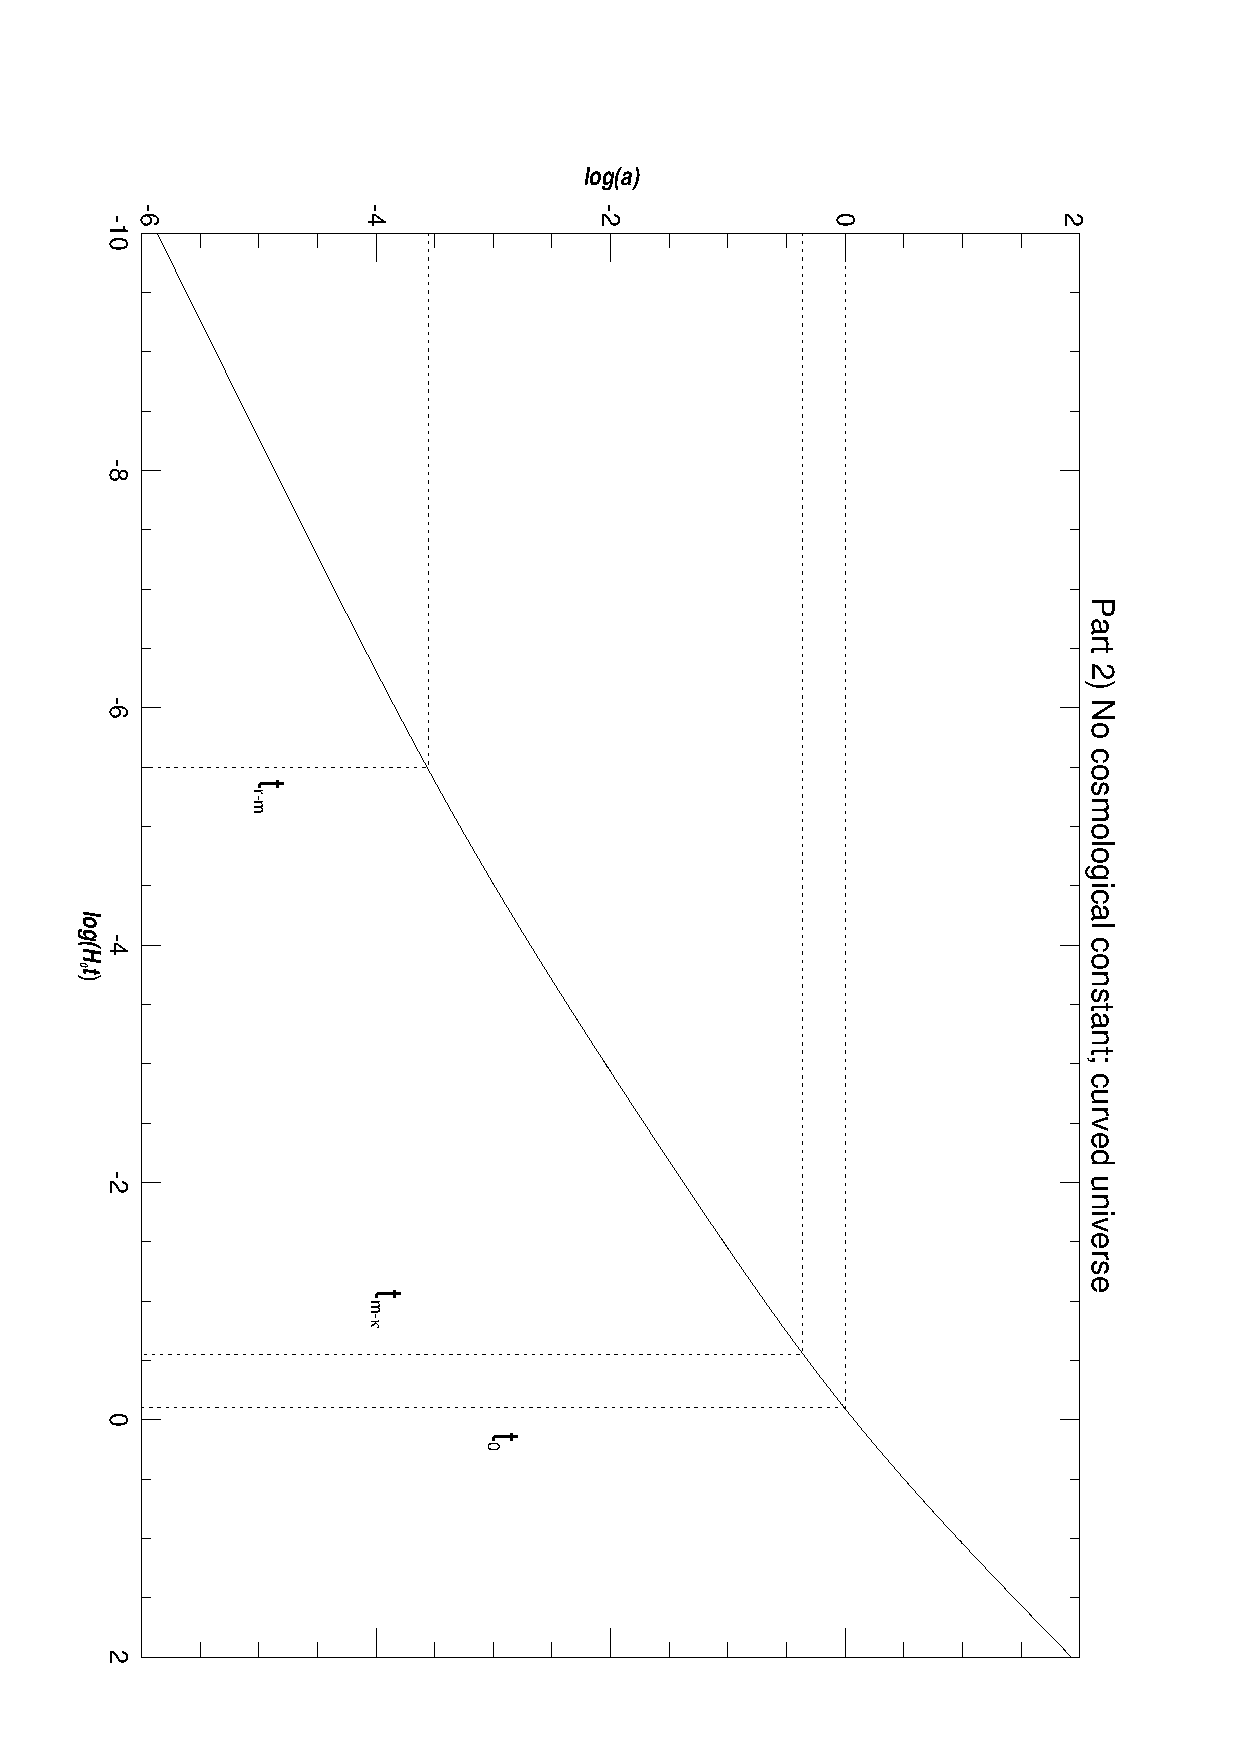
\includegraphics[scale=0.6]{advanced_part2.pdf}}

\newpage
%\vspace*{0.5cm}
\item[\textbf{Part 3.}]

The last measurements of the curvature of the universe indicate that the density parameter is $\Omega=1.02 \pm 0.02$. Integrate again the equation (\ref{HLlaw}) with $\Omega_{m,0}=0.32$ and $\Omega_{\Lambda,0}=0.7$, and then with $\Omega_{m,0}=0.3$ and $\Omega_{\Lambda,0}=0.72$.

\vspace{0.5cm}
\textbf{Solution:}
Once again, modify the constants of the program in Part 1, and plot the results as $(\log(H_0 t),\log(a))$ for the two universes.

\vspace*{0.5cm}
\textbf{Results:}

The final plot $(\log(H_0 t),\log(a))$, with radiation-matter equality $t_{r-m}$, matter-cosmological constant equality $t_{m-\Lambda}$, and the present moment $t_0$ included.

\centerline{\includegraphics[scale=0.6]{advanced_part3a.pdf}}


\centerline{\includegraphics[scale=0.6]{advanced_part3b.pdf}}

\newpage
%\vspace*{0.5cm}
\item[\textbf{Part 4.}]

Comment about the differences in the scale factor evolution of the four universe models that you just integrated.

\vspace{0.5cm}
\textbf{Results from the plots:}

For the benchmark model, in the logarithmic scale:
$$a_{r-m}=-3.5528420, \,\,\, H_0 t_{r-m} = -5.5$$ 
$$a_{m-\Lambda}=-0.12493874, \,\,\, H_0 t_{m-\Lambda} = -0.15$$ 
$$a(t_0)=0, \,\,\, H_0 t_0 = 0$$

For the $\Omega_{\Lambda,0}=0$ case, in the logarithmic scale:
$$a_{r-m}=-3.5528420, \,\,\, H_0 t_{r-m} = -5.5$$ 
$$ a_{m-\kappa}=-0.36792467,  \,\,\, H_0 t_{m-\kappa} = -0.55$$ 
$$a(t_0)=0, \,\,\, H_0 t_0 = -0.1$$

For the $\Omega_{m,0}=0.32$, $\Omega_{\Lambda,0}=0.7$ case, in the logarithmic scale:
$$a_{r-m}=-3.5808707, \,\,\, H_0 t_{r-m} = -5.55$$
$$a_{m-\Lambda}=-0.11331602, \,\,\, H_0 t_{m-\Lambda} = -0.15$$
$$a(t_0)=0, \,\,\, H_0 t_0 = -0.015$$

For the $\Omega_{m,0}=0.3$, $\Omega_{\Lambda,0}=0.72$ case, in the logarithmic scale:
$$a_{r-m}=-3.5528420, \,\,\, H_0 t_{r-m} = -5.5$$
$$a_{m-\Lambda}=-0.12673708, \,\,\, H_0 t_{m-\Lambda} = -0.15$$ 
$$a(t_0)=0, \,\,\, H_0 t_0 = 0$$


\vspace{0.5cm}
\textbf{Answer part 1: Benchmark model and the $\Omega_{\Lambda,0}=0$ -modification}

For the first two models, i.e. the benchmark model and the universe without cosmological constant, the radiation-matter equality happens at the same time, and $a=a_{r-m}$ is the same in both cases.

Between $a=0$ and $a=a_{r-m}$ the scale factor grows proportional to $a \propto t^{1/2}$ in both of the models.

In the second model the cosmological constant is absent, so there is no $a_{m-\Lambda}$. Also, the present moment is located slightly more to the left compared to the first model. For the benchmark model $\log(H_0 t_0) = 0$, but in the second model $\log(H_0 t_0) = -0.1$. 
This means that in the $\Omega_{\Lambda,0}=0$ case the current age of the universe is smaller than in the benchmark model.

Between $a=a_{r-m}$ and $a=1$ the scale factor grows nearly identically as $a \propto t^{2/3}$ in both models.

In the benchmark model the scale factor $a$ grows exponentially as $a \propto e^{Kt}$ after the $a_{m-\Lambda}$ -limit ($\log(a_{m-\Lambda})=-0.12493874$), which is located close to the present time $(\log(a)=0)$. 

In the universe without cosmological constant, the growth of the scale factor after the present time is not nearly as explosive as in the benchmark model. Since $(1-\Omega_0)>0$, the negative curvature $\kappa$ acts like a third component for the universe.
At the limit $\log(a_{m-\kappa})=-0.36792467$, when the corresponding time is $\log(H_0 t_{m-\kappa})=-0.55$, the universe changes from a matter-dominated universe into a curvature-dominated one. After the limit $a_{m-\kappa}$, the scale factor grows as $a \propto t$.
%Instead, the increase rate of $a$ stays the same as in the time between $a_{r-m}$ and $a=1$.

\vspace{0.5cm}
\textbf{Answer part 2: Benchmark model and its corrections}

The last two models are possible corrections to the benchmark model. Both are very similar to each other, and the evolution of the scale factor is nearly the same as in the benchmark model.
However, as the plots are logarithmic, even the small differences may be important.

The differences in the slope of $a$ between the models are not well distinguishable with naked eye, but the variation of the different epochs is more easily seen.

In the $\Omega_{m,0}=0.32$, $\Omega_{\Lambda,0}=0.7$ -universe, the radiation-matter equality happens slightly earlier than in the benchmark model, and $a_{r-m}$ is smaller. 
In the $\Omega_{m,0}=0.3$, $\Omega_{\Lambda,0}=0.72$ -model, the time and scale factor of the radiation-matter equality are exactly the same as in the benchmark model.

The mass-cosmological constant equality happens at the same time in the $\Omega_{m,0}=0.32$, $\Omega_{\Lambda,0}=0.7$ -model than it does in the benchmark model, but the scale factor $a_{m-\Lambda}$ is larger.

In the $\Omega_{m,0}=0.3$, $\Omega_{\Lambda,0}=0.72$ -model the mass-cosmological constant equality also happens at the same time than it does in the benchmark model, but the scale factor $a_{m-\Lambda}$ is smaller.

The current age of the universe is smaller in the $\Omega_{m,0}=0.32$, $\Omega_{\Lambda,0}=0.7$ -model than in the benchmark model. In the $\Omega_{m,0}=0.3$, $\Omega_{\Lambda,0}=0.72$ -model the age of the universe is the same as in the benchmark model.

\newpage
%\vspace*{0.5cm}
\item[\textbf{Part 5.}]

One of the reasons why a precise calibration of the benchmark model is necessary is to be able to find a lookback time from redshift. In that way, we can study with detail the evolution with time of galaxies. Plot the lookback time as a function of redshift for all the four models that you just computed (like in the lecture notes Ch5, page 14).

\vspace{0.5cm}

\textbf{Solution:}

Function for solving the first Friedmann equation:

\begin{scriptsize}
\begin{verbatim}
;------------------------------------------------------------------;
; friedmann.pro
;------------------------------------------------------------------;
; Description:
; Function for solving the first Friedmann equation for a
; multi-component universe.
; Creates vector a and solves h0t for those values of a.
; Uses given values for energy densities in solving the 
; 1st Friedmann equation.

; Input: 
;   relative energy densities as a vector
;   (om_r0,om_m0,om_l0)
; = (radiation, mass, cosmological constant)
; Output: array (h0t,a)
;--------------------------------------------------------------------;
function friedmann,densities

;Take relative energy densities from the input
;Radiation
om_r0=densities(0)
;Mass
om_m0=densities(1)
;Cosmological constant
om_l0=densities(2)
;Total:
om_0=om_r0+om_m0+om_l0
;----------------------------------------------------------------------;
; Scale factor:
;----------------------------------------------------------------------;
; Reduce the total steps needed by increasing stepsize as a increases.
; For the purpose of the last cosmology assignment, I modified a so 
; that it  ends at the present time a=1.
; This is useful for determining lookback times.

; Between a=0 and a=0.001 (1000 steps)
a1=findgen(1000)*0.000001d0
; Between a=0.001 and a=0.01 (900 steps)
a2=findgen(900)*0.00001d0+0.001d
; Between a=0.01 and a=0.1 (900 steps)
a3=findgen(900)*0.0001d0+0.01d0
; Between a=0.1 and a=1 (901 steps)
a4=findgen(901)*0.001d0+0.1d0

; Between a=0.1 and a=1 (900 steps)
;a4=findgen(900)*0.001d0+0.1d0
; Between a=1 and a=10 (900 steps)
;a5=findgen(900)*0.01d0+1.d0
; Between a=10 and a=100 (900 steps)
;a6=findgen(900)*0.1d0+10.d0

; Different parts combined:
a=[a1,a2,a3,a4]
;a=[a1,a2,a3,a4,a5,a6]

;----------------------------------------------------------------------;
; Time:
;----------------------------------------------------------------------;
n=n_elements(a)
h0t=findgen(n)*0.0d0

;----------------------------------------------------------------------;
; H-L law
;----------------------------------------------------------------------;
;Make a loop that solves h0t[n] from a[n] and saves the results to
;the vector h0t

;Starting values
i=1
h0t[0]=0.0d0

; The loop:
while i lt n do begin
; Define da
   da=a[i]-a[i-1]
; Use midpoint rule for a
   a_temp=(a[i]+a[i-1])/2.d0
; Actual equation
   h0t[i]=h0t[i-1] + (om_r0/a_temp^2+om_m0/a_temp+om_l0*a_temp^2+(1-om_0))^(-1/2.d0)*da
; Increase index i
   i=i+1
endwhile

;Result array is [[h0t],[a]]
result=[[h0t],[a]]

return,result
end
\end{verbatim}
\end{scriptsize}

\vspace{0.5cm}

The main program for determining lookback times for objects of different redshifts:

\begin{scriptsize}
\begin{verbatim}
;------------------------------------------------------------------------;
; Introduction to cosmology - Computer assignment for advanced students
;------------------------------------------------------------------------;
;  PART V
;------------------------------------------------------------------------;
; Use the subroutine PsPlot to save results in a postscript plot 
; (written by Heikki Salo)
;------------------------------------------------------------------------;
pro PsPlot,routine,filename
	thisdir=getenv('PWD')+'/'
	psopen,/color,dir=thisdir,filename
	call_procedure,routine
	psclose		
end
;------------------------------------------------------------------------;

;------------------------------------------------------------------------;
;  MAIN PROGRAM starts here
;------------------------------------------------------------------------;
; Plot the lookback time (t0-te) as a function of redshift z for the
; four models that were computed in parts 1-3 of the assignment.

pro advanced_part5

;------------------------------------------------------------------------;
;  Constant(s)
;------------------------------------------------------------------------;
;H-L constant (km/Mpc)/s
;h0=70

;Can't use 1/s unit, in which h0 would be
;h0=70.d0/(3.08567756d0)*10^(-19)
;so a unit transformation is needed at a later point when solving times

; Use 10^(-19) 1/s as the unit
h0=70.d0/(3.08567756d0)

;------------------------------------------------------------------------;
;  1st Friedmann equation
;------------------------------------------------------------------------;
; Use the function 'friedmann' to solve the first Friedmann equation
; for different universes.
; Input: vector of relative energy densities [om_r0,om_m0,om_l0]
; Output: array result=[[h0t],[a]]

;-----------------------------------------------------------------------;
; 1st Friedmann) First model: benchmark
;-----------------------------------------------------------------------;
; Radiation:
om_r01=8.4d0*10^(-5.d0)
; Mass:
om_m01=0.3d0
; Cosmological constant:
om_l01=0.7d0

result1=friedmann([om_r01,om_m01,om_l01])

;Separate a and h0t from each other
h0t1=result1[*,0]
a1=result1[*,1]

;-----------------------------------------------------------------------;
;  1st Friedmann) Second model: no cosmological constant
;-----------------------------------------------------------------------;
; Radiation:
om_r02=8.4d0*10^(-5.d0)
; Mass:
om_m02=0.3d0
; Cosmological constant:
om_l02=0.d0

result2=friedmann([om_r02,om_m02,om_l02])

;Separate a and h0t from each other
h0t2=result2[*,0]
a2=result2[*,1]

;-----------------------------------------------------------------------;
;  1st Friedmann) Third model
;-----------------------------------------------------------------------;
; Radiation:
om_r03=8.4d0*10^(-5.d0)
; Mass:
om_m03=0.32d0
; Cosmological constant:
om_l03=0.7d0

result3=friedmann([om_r03,om_m03,om_l03])

;Separate a and h0t from each other
h0t3=result3[*,0]
a3=result3[*,1]

;-----------------------------------------------------------------------;
;  1st Friedmann) Fourth model
;-----------------------------------------------------------------------;
; Radiation:
om_r04=8.4d0*10^(-5.d0)
; Mass:
om_m04=0.3d0
; Cosmological constant:
om_l04=0.72d0

result4=friedmann([om_r04,om_m04,om_l04])

;Separate a and h0t from each other
h0t4=result4[*,0]
a4=result4[*,1]

;-----------------------------------------------------------------------;
;  Lookback time (t0-te)
;-----------------------------------------------------------------------;
;-----------------------------------------------------------------------;
; Times of emission te are taken from h0t -vectors
;-----------------------------------------------------------------------;
; First model (benchmark)
te1=h0t1/h0

;Second model
te2=h0t2/h0

;Third model
te3=h0t3/h0

;Fourth model
te4=h0t4/h0

;-----------------------------------------------------------------------;
; Present time t0 is when a=1
;-----------------------------------------------------------------------;
; Last element of vector a is a=1, so the present time t0 is the last 
; element  of the corresponding time vector te.

index=n_elements(a1)-1

;First model
t01=te1[index]
;Second model
t02=te2[index]
;Third model
t03=te3[index]
;Fourth model
t04=te4[index]

;--------------------------------------------------------------------;
; Redshift z for the different models
;--------------------------------------------------------------------;
; Redshift can be solved from a(te):
; (1+z)=a(t0)/a(te) -> z=1/a(te)-1
; Result is a vector of the same lenght as a and te.

; First model (benchmark)
z1=1.d0/a1-1

; 2nd model
z2=1.d0/a2-1

; 3rd model
z3=1.d0/a3-1

; 4th model
z4=1.d0/a4-1

;--------------------------------------------------------------------;
; Plot the lookback times (t0-te) as a function of redshift z
;--------------------------------------------------------------------;
; Note: the original unit for the times is 10^19 s because of the 
; chosen unit for H-L constant

; Change to Gy (10^9 years)
; 1 Gy = 10^9*365*24*60^2 s = 3.1536*10^16 s
; so 10^19 s = 317.0979198 Gy

;---------------------------------------------------------------------;
; First model: Benchmark
;---------------------------------------------------------------------;
t_lb1=(t01-te1)*317.0979198

nwin
plot,z1,t_lb1,title='Model 1) Benchmark',xtitle='z',ytitle='t!I0!N-t!Ie!N (Gyr)',xrange=[0,15],yrange=[0,15],charsize=1.5
oplot,[11.9,11.9],[0,13.1],linestyle=1
oplot,[0,11.9],[13.1,13.1],linestyle=1
xyouts, 5,13.5, '(t!I0!N-t!Ie!N)=13.1', charsize=1.5
xyouts, 12.1,7, 'z=11.9', charsize=1.5

;---------------------------------------------------------------------;
; Second model: om_l0=0
;---------------------------------------------------------------------;
t_lb2=(t02-te2)*317.0979198

nwin
plot,z2,t_lb2,title='Model 2) !9W!IL!X,0!N=0',xtitle='z',ytitle='t!I0!N-t!Ie!N (Gyr)',xrange=[0,15],yrange=[0,15],charsize=1.5
oplot,[11.9,11.9],[0,10.95],linestyle=1
oplot,[0,11.9],[10.95,10.95],linestyle=1
xyouts, 5,11.5, '(t!I0!N-t!Ie!N)=10.95', charsize=1.5
xyouts, 12.1,7, 'z=11.9', charsize=1.5

;---------------------------------------------------------------------;
; Third model: om_m0=0.32,om_l0=0.7
;---------------------------------------------------------------------;
t_lb3=(t03-te3)*317.0979198

nwin
plot,z3,t_lb3,title='Model 3) !9W!I!Xm,0!N=0.32, !9W!IL!X,0!N=0.7',xtitle='z',ytitle='t!I0!N-t!Ie!N (Gyr)',xrange=[0,15],yrange=[0,15],charsize=1.5
oplot,[11.9,11.9],[0,12.95],linestyle=1
oplot,[0,11.9],[12.95,12.95],linestyle=1
xyouts, 5,13.4, '(t!I0!N-t!Ie!N)=12.95', charsize=1.5
xyouts, 12.1,7, 'z=11.9', charsize=1.5

;---------------------------------------------------------------------;
; Fourth model: om_m0=0.3,om_l0=0.72
;---------------------------------------------------------------------;
t_lb4=(t04-te4)*317.0979198

nwin
plot,z4,t_lb4,title='Model 4) !9W!I!Xm,0!N=0.3, !9W!IL!X,0!N=0.72',xtitle='z',ytitle='t!I0!N-t!Ie!N (Gyr)',xrange=[0,15],yrange=[0,15],charsize=1.5
oplot,[11.9,11.9],[0,13.2],linestyle=1
oplot,[0,11.9],[13.2,13.2],linestyle=1
xyouts, 5,13.5, '(t!I0!N-t!Ie!N)=13.2', charsize=1.5
xyouts, 12.1,7, 'z=11.9', charsize=1.5

end

;--------------------------------------------------------------------;
; Save the results to a PostScript file using PsPlot
;--------------------------------------------------------------------;
pro Plot_everything5
PsPlot, 'advanced_part5', 'advanced_part5.ps'
end
\end{verbatim}
\end{scriptsize}

\vspace*{1cm}
\textbf{Results:}

Lookback time $(t_0-t_e)$ in gigayears as a function of the redshift $z$.

%\vspace*{-0.5cm}
\centerline{\includegraphics[scale=0.6]{advanced_part5a.pdf}}

\centerline{\includegraphics[scale=0.6]{advanced_part5b.pdf}}

\centerline{\includegraphics[scale=0.6]{advanced_part5c.pdf}}

\centerline{\includegraphics[scale=0.6]{advanced_part5d.pdf}}

\newpage
\vspace*{0.5cm}
\item[\textbf{Part 6.}]

To the date, the farthest known galaxy is found at $z=11.9$. What is its lookback time according to the four models that you have studied?

\vspace*{0.5cm}
\textbf{Model 1}
In the benchmark model the lookback time $(t_0-t_e)$ for a galazy of redshift $z=11.9$ is about $13.1\text{Gyr}$.

\centerline{\includegraphics[scale=0.6]{advanced_part6a.pdf}}

\vspace*{0.5cm}
\newpage
\textbf{Model 2}
In the $\Omega_{\Lambda,0}=0$ -model the lookback time $(t_0-t_e)$ for a galazy of redshift $z=11.9$ is about $10.95\text{Gyr}$.

\centerline{\includegraphics[scale=0.6]{advanced_part6b.pdf}}

\vspace*{0.5cm}
\newpage
\textbf{Model 3}
In the $\Omega_{m,0}=0.32, \Omega_{\Lambda,0}=0.7$ -model the lookback time $(t_0-t_e)$ for a galazy of redshift $z=11.9$ is about $12.95\text{Gyr}$.

\centerline{\includegraphics[scale=0.6]{advanced_part6c.pdf}}

\vspace*{0.5cm}
\newpage
\textbf{Model 4}
In the $\Omega_{m,0}=0.3, \Omega_{\Lambda,0}=0.72$ -model the lookback time $(t_0-t_e)$ for a galazy of redshift $z=11.9$ is about $13.2\text{Gyr}$.

\centerline{\includegraphics[scale=0.6]{advanced_part6d.pdf}}

\end{itemize}

\end{document}